% Paper skeleton. Section bodies are intentionally EMPTY.
%
% Two workspace rules shape this file:
%   * rule 1 -- no number may appear that did not come from code that actually ran, so every
%     table is \input from paper/tables/, which code/make_tables.py regenerates from results/.
%   * rule 7 -- the author reads and approves every section, so prose is written one section at a
%     time and nothing is drafted ahead of the evidence.
%
% Target venue: ISSTA 2027 Research Papers (mandatory abstract 2027-01-08 AoE, full paper
% 2027-01-11 AoE; checked on 2026-10-12 at
% https://conf.researchr.org/track/issta-2027/issta-2027-research-papers).
% On that date the ISSTA 2027 CFP body was still "TBD", so the page limit, template and
% anonymity rules MUST be re-checked before submission. This skeleton therefore uses the ACM
% sigconf style used by SIGSOFT venues; switching to IEEEtran is a small change if needed.
%
% Compile: see paper/README.md

% `review` is deliberately NOT used. It switches on acmart's line numbering, and those numbers are
% printed down the page margin straight over the floats, so every table and figure arrives with a
% column of line numbers across it. Anonymity is kept for submission; the venue metadata is set so
% the header names ISSTA rather than acmart's placeholder conference.
\documentclass[sigconf,anonymous]{acmart}

\setcopyright{none}
\settopmatter{printacmref=false}
\renewcommand\footnotetextcopyrightpermission[1]{}
\pagestyle{plain}

\acmConference[ISSTA 2027]{International Symposium on Software Testing and Analysis}{September 2027}{Singapore}
\acmYear{2027}

\usepackage{booktabs}
\usepackage{graphicx}

% Inline code appears constantly in this paper (`specific_reassign`,
% `results/history_verification.json`), and by default a \texttt run cannot be hyphenated, so those
% words overflow a column and print over the neighbouring one. `htt` turns hyphenation on inside
% \texttt; the extra emergencystretch lets a line stretch a little before it overflows.
\usepackage[htt]{hyphenat}
\setlength{\emergencystretch}{2em}

% Every figure the prose quotes is a macro generated by code/make_tables.py from results/. The
% sweep adds bugs day by day, so a hard-coded number in the text would silently disagree with the
% table it cites; these cannot.
% Generated by code/make_tables.py from results/metrics_*.json.
% Every figure the prose quotes lives here, so text and tables cannot drift apart.
% Regenerate after each day of the sweep:  python code/make_tables.py --split test2026

\newcommand{\nAgentN}{6{,}347}
\newcommand{\nAgentAcc}{78.9}
\newcommand{\nAgentTop}{93.5}
\newcommand{\nAgentAurc}{0.077}
\newcommand{\nAgentCov}{86.2}
\newcommand{\nAgentSpecN}{656}
\newcommand{\nAgentSpecAcc}{71.2}
\newcommand{\nAgentNeverAcc}{80.0}
\newcommand{\nAgentLift}{1.13}
\newcommand{\nAgentErrInit}{49.7}
\newcommand{\nAgentSpecAbst}{22.6}
\newcommand{\nAgentNeverAbst}{19.0}
\newcommand{\nAgentUsd}{0.0047}
\newcommand{\nAgentLat}{5.09}
\newcommand{\nAgentCalls}{3.57}
\newcommand{\nAgentInTok}{30{,}214}
\newcommand{\nAgentGap}{8.8}
\newcommand{\nZSN}{6{,}347}
\newcommand{\nZSAcc}{70.9}
\newcommand{\nZSTop}{88.4}
\newcommand{\nZSAurc}{0.157}
\newcommand{\nZSCov}{76.1}
\newcommand{\nZSSpecN}{656}
\newcommand{\nZSSpecAcc}{63.7}
\newcommand{\nZSNeverAcc}{72.4}
\newcommand{\nZSLift}{0.69}
\newcommand{\nZSErrInit}{35.3}
\newcommand{\nZSSpecAbst}{13.9}
\newcommand{\nZSNeverAbst}{20.5}
\newcommand{\nZSUsd}{0.0014}
\newcommand{\nZSLat}{1.77}
\newcommand{\nZSCalls}{0.00}
\newcommand{\nZSInTok}{9{,}254}
\newcommand{\nZSGap}{8.7}
\newcommand{\nRagN}{6{,}347}
\newcommand{\nRagAcc}{68.0}
\newcommand{\nRagTop}{87.7}
\newcommand{\nRagAurc}{0.176}
\newcommand{\nRagCov}{73.7}
\newcommand{\nRagSpecN}{656}
\newcommand{\nRagSpecAcc}{61.1}
\newcommand{\nRagNeverAcc}{68.9}
\newcommand{\nRagLift}{0.88}
\newcommand{\nRagErrInit}{37.6}
\newcommand{\nRagSpecAbst}{17.7}
\newcommand{\nRagNeverAbst}{19.9}
\newcommand{\nRagUsd}{0.0018}
\newcommand{\nRagLat}{1.69}
\newcommand{\nRagCalls}{0.00}
\newcommand{\nRagInTok}{11{,}532}
\newcommand{\nRagGap}{7.8}
\newcommand{\nRepN}{6{,}347}
\newcommand{\nRepAcc}{83.1}
\newcommand{\nRepTop}{87.4}
\newcommand{\nRepAurc}{0.333}
\newcommand{\nRepCov}{82.7}
\newcommand{\nRepSpecN}{656}
\newcommand{\nRepSpecAcc}{32.8}
\newcommand{\nRepNeverAcc}{100.0}
\newcommand{\nRepLift}{1.65}
\newcommand{\nRepErrInit}{84.8}
\newcommand{\nRepSpecAbst}{33.1}
\newcommand{\nRepNeverAbst}{21.2}
\newcommand{\nRepUsd}{--}
\newcommand{\nRepLat}{0.00}
\newcommand{\nRepCalls}{0.00}
\newcommand{\nRepInTok}{0}
\newcommand{\nRepGap}{67.2}
\newcommand{\nLrN}{6{,}347}
\newcommand{\nLrAcc}{62.5}
\newcommand{\nLrTop}{84.4}
\newcommand{\nLrAurc}{0.184}
\newcommand{\nLrCov}{69.9}
\newcommand{\nLrSpecN}{656}
\newcommand{\nLrSpecAcc}{55.6}
\newcommand{\nLrNeverAcc}{63.0}
\newcommand{\nLrLift}{0.84}
\newcommand{\nLrErrInit}{29.6}
\newcommand{\nLrSpecAbst}{16.8}
\newcommand{\nLrNeverAbst}{21.3}
\newcommand{\nLrUsd}{--}
\newcommand{\nLrLat}{0.00}
\newcommand{\nLrCalls}{0.00}
\newcommand{\nLrInTok}{0}
\newcommand{\nLrGap}{7.4}
\newcommand{\nXgbN}{6{,}347}
\newcommand{\nXgbAcc}{59.6}
\newcommand{\nXgbTop}{82.1}
\newcommand{\nXgbAurc}{0.196}
\newcommand{\nXgbCov}{67.7}
\newcommand{\nXgbSpecN}{656}
\newcommand{\nXgbSpecAcc}{52.9}
\newcommand{\nXgbNeverAcc}{60.2}
\newcommand{\nXgbLift}{0.69}
\newcommand{\nXgbErrInit}{27.5}
\newcommand{\nXgbSpecAbst}{13.9}
\newcommand{\nXgbNeverAbst}{21.6}
\newcommand{\nXgbUsd}{--}
\newcommand{\nXgbLat}{0.00}
\newcommand{\nXgbCalls}{0.00}
\newcommand{\nXgbInTok}{0}
\newcommand{\nXgbGap}{7.3}
\newcommand{\nAgentOverLr}{16.4}
\newcommand{\nAgentSpecOverLr}{15.5}
\newcommand{\nAgentSpecOverRep}{38.4}
\newcommand{\nClassicalLiftMin}{0.69}
\newcommand{\nClassicalLiftMax}{0.90}
\newcommand{\nNonFirefoxGeneral}{68}
\newcommand{\nReviewN}{150}
\newcommand{\nReviewAgree}{100.0}
\newcommand{\nReviewKappa}{1.00}
\newcommand{\nVerifyN}{150}
\newcommand{\nVerifyMatch}{150}
\newcommand{\nVerifyExtra}{0}
\newcommand{\nVerifyMismatch}{0}
\newcommand{\nSharedN}{6{,}347}
\newcommand{\nAgentOnly}{1{,}383}
\newcommand{\nLrOnly}{342}
\newcommand{\nNetNever}{17.0}
\newcommand{\nNetMoved}{15.6}
\newcommand{\nLossOne}{259}
\newcommand{\nLossTwo}{108}
\newcommand{\nLossThree}{68}

\begin{document}

\title{Selective Routing under Ownership Ambiguity:\\
A Public Benchmark and an Agent Study}

\author{Anonymous submission}
\affiliation{%
  \institution{Independent Researcher}
  \country{}}

\begin{abstract}
% Every number here also appears in Table~\ref{tab:conditions-test2026} or
% Table~\ref{tab:ambiguity-test2026}, as the workspace rules require.
Bug reports are routed by hand: a reporter picks a component, a triager moves it when that choice
was wrong, and the component decides which team fixes the bug. We show that the usual way of
scoring this task hides the only part of it that is hard. On a public Mozilla Bugzilla benchmark,
simply predicting the team that owns the component the reporter already chose reproduces the final
team for \nRepAcc\% of the bugs, more than any trained model we tried (best: \nLrAcc\%). That
figure is earned on reports that were never reassigned, where the same baseline scores
\nRepNeverAcc\%; on reports that were moved away from a concrete component it collapses to
\nRepSpecAcc\%, below the \nLrSpecAcc\% of TF-IDF with logistic regression. Overall accuracy
therefore rewards the method that adds least.

We then ask whether a tool-using LLM agent can do better exactly there. On the same bugs the agent
reaches \nAgentAcc\% overall and \nAgentSpecAcc\% on the reassigned subgroup --- \nAgentSpecOverLr
points above the best classical model and \nAgentSpecOverRep{} points above the reporter baseline ---
with the best risk-coverage curve of any method we evaluate (AURC \nAgentAurc, against \nLrAurc{} for
TF-IDF with logistic regression and \nRepAurc{} for the reporter baseline). It is also the one learned
method that declines more often on the reassigned bugs than elsewhere, \nAgentSpecAbst\% against
\nAgentNeverAbst\%, a lift of \nAgentLift, where every classical method declines on them at
\nClassicalLiftMin--\nClassicalLiftMax{} times its own average rate. That margin is narrower than the accuracy gain, and we report
it as such. We release the benchmark, the baselines and the prompts.
\end{abstract}

\maketitle

\section{Introduction}
% DRAFT for author review (rule 7). The numbers quoted here all appear in
% Table~\ref{tab:conditions-test2026} and Table~\ref{tab:ambiguity-test2026}; no number in this
% section is typed from anywhere else.

Bug reports are routed by hand. A reporter picks a component, a triager moves the report when
that choice was wrong, and the component decides which team eventually fixes it. A routing
decision can therefore fail in two ways: the report was filed under the wrong component, or the
right component is hard to identify from the text.

Prior work treats routing as text classification and reports overall accuracy
\cite{sarkar2019ericsson,su2021bugtossing,dipongkor2023comparative,su2023stillconfusing,mamun2026triagerx}.
On our data that framing is misleading. The strongest signal available at filing time is the
component the reporter already chose: predicting the team that owns it reproduces the final team
for \nRepAcc\% of the bugs in our 2026 test period, against \nLrAcc\% for TF-IDF with logistic
regression and less for every other trained model we tried
(Table~\ref{tab:conditions-test2026}). An accuracy leaderboard would conclude that routing is
nearly solved and that no trained model is worth deploying. Production systems take the same
view: BugBug in Firefox applies a confidence threshold and assigns only what it is sure of
\cite{castelluccio2019bugbug}.

The aggregate hides the only subgroup where a model helps. Splitting those same bugs by whether
their component ever moved shows that the reporter baseline collapses exactly where routing is
hard: \nRepNeverAcc\% on bugs that were never reassigned, but \nRepSpecAcc\% on the bugs that were
moved away from a concrete component, where TF-IDF+LR reaches \nLrSpecAcc\%
(Table~\ref{tab:ambiguity-test2026}). The baseline's 83\% is earned almost entirely on the easy
majority of reports.

The second half of the problem is that the classical methods cannot tell when they are wrong.
Ranking bugs by a trained model's confidence and answering only the most confident fraction does
raise its accuracy, but every classical method declines on the reassigned subgroup at only
\nClassicalLiftMin--\nClassicalLiftMax{} times the rate at which it declines overall: it answers the hard bugs \emph{more}
readily than the easy ones (Table~\ref{tab:ambiguity-test2026}). Its confidence does not track the
ambiguity it would need to detect. The reporter baseline is the other exception (lift \nRepLift), and
only because its confidence is a class prior rather than a text-based estimate.

That is the question this paper asks. Can an LLM agent, given tools and asked for candidate teams
with evidence, identify ambiguous reports better than a confidence threshold can? Recent systems
route incidents with single LLMs \cite{wang2024comet}, with several agents that negotiate
\cite{yu2025triangle}, and with one agent per team \cite{yao2026agentic}; abstention has been used
to cut noise in agentic program repair \cite{cambronero2026abstain}. We answer the question on
public data with a benchmark, a set of strong baselines, and three abstention mechanisms.

\paragraph{What we find.}
The agent does better exactly where the task is hard. It reaches \nAgentAcc\% overall and
\nAgentSpecAcc\% on the reassigned bugs, against \nLrSpecAcc\% for the best classical model and
\nRepSpecAcc\% for the reporter baseline, and it has the best risk-coverage curve of any method we
evaluate (AURC \nAgentAurc{} against \nLrAurc). Its abstention points the right way, but only just: a
lift of \nAgentLift, against \nClassicalLiftMin--\nClassicalLiftMax{} for every classical method
(Table~\ref{tab:ambiguity-test2026}). Retrieval is not what earns the accuracy. Single-round RAG is
the weakest of the three LLM conditions at \nRagAcc\%, below the \nZSAcc\% the same model reaches
with no retrieval at all (Table~\ref{tab:conditions-test2026}); it is the tool loop, not the extra
context, that helps.

\paragraph{Contributions.}
\begin{itemize}
\item A public benchmark for team-level routing built from the Bugzilla API, with two test periods
and a weak label for ownership ambiguity derived from reassignment history
(Section~\ref{sec:data}).
\item The observation that the component the reporter already chose is the strongest single signal
(\nRepAcc\%) and that overall accuracy therefore hides the subgroup where routing is actually hard,
together with the per-category accuracy and abstention analysis that exposes it
(Table~\ref{tab:ambiguity-test2026}).
\item Eight classical baselines and three LLM conditions scored by one evaluator, showing that a
tool-using agent is both the most accurate method on the reassigned subgroup (\nAgentSpecAcc\%) and
the only learned method whose abstention points the right way there, by a margin narrower than its
accuracy gain (lift \nAgentLift).
\item A cost and configuration study from measured token counts, including the measurement that
the model's thinking mode buys no accuracy on this task while multiplying output tokens by five to
nineteen (Table~\ref{tab:thinking-deepseek-flash}).
\end{itemize}

\section{Related Work}
\label{sec:related}

% DRAFT for author review (rule 7). Every citation below is a verified entry in
% shared/references.bib (rule 2); none is cited from memory.

\paragraph{Routing as classification.}
Component and developer assignment has been studied as text classification for two decades.
Sarkar et al.\ found at Ericsson that a classifier is accurate enough to be useful only above a
high confidence threshold, and that everything below it should go to a human
\cite{sarkar2019ericsson}. BugBug, in production for Firefox, applies the same idea with a 60\%
threshold over an XGBoost model \cite{castelluccio2019bugbug}. Later work adds structure to the
text: Su et al.\ learn from earlier misroutes with a bug-tossing knowledge graph
\cite{su2021bugtossing}, and single out confusable components by distinguishing reports that were
reassigned from those that were not \cite{su2023stillconfusing}. Transformer representations
improve on TF-IDF \cite{dipongkor2023comparative}, and ensembles of fine-tuned models improve
further \cite{dipongkor2024ensemble}. We keep this line of work as baselines (TF-IDF, embeddings,
XGBoost) and add the signal these papers do not compare against: the component the reporter
already chose.

\paragraph{Agentic and LLM triage.}
Instruction-tuned models with constrained decoding reach a Hit@10 of 0.753 while exact top-1
accuracy stays modest \cite{kiashemshaki2025instruction}, and a benchmark of classical,
transformer and RAG approaches finds the classical models hard to beat
\cite{lajko2026benchmarking}. TriagerX reports a deployment in which components act as proxies for
teams \cite{mamun2026triagerx}. In incident triage, a single LLM assigns incidents to teams with an
explanation \cite{wang2024comet}, several agents negotiate an assignment \cite{yu2025triangle}, and
one agent per team decides whether to accept it \cite{yao2026agentic}; TianoForge does the same for
firmware reports \cite{siavash2026tianoforge}. These systems are compared by assignment accuracy.
Our claim is that aggregate accuracy is the wrong summary for this task, so we measure the same
kind of system on the subgroup where ownership actually moved.

\paragraph{Abstention and selective prediction.}
Declining to answer is an old idea: Chow derived the optimal error-reject tradeoff
\cite{chow1970optimum}, selective classification was later put on a risk-coverage footing
\cite{elyaniv2010foundations} and extended to neural networks with a guaranteed risk
\cite{geifman2017selective}. Conformal prediction gives candidate sets with distribution-free
coverage \cite{angelopoulos2021gentle}, which is what our prediction-set baseline uses. In software
engineering, abstention has recently been used to cut the noise produced by agentic program repair
\cite{cambronero2026abstain}. We keep the risk-coverage framing and apply it to a label whose noise
is not random: here the ambiguity comes from the ownership history of the bug.

\paragraph{Data and surveys.}
Our corpus is built directly from the public Bugzilla API. GitBugs aggregates Bugzilla, GitHub and
Jira reports for related tasks \cite{patil2025gitbugs}, and a systematic review of 234 triage
papers surveys the field and its evaluation practices \cite{zhao2025triage}.

\section{Data and ownership-ambiguity labels}
\label{sec:data}

% DRAFT for author review (rule 7). Every number below was produced by the scripts named next to
% it; the category counts are in Table~\ref{tab:categories}.

\paragraph{Corpus.}
We read the public Mozilla Bugzilla REST API. A bug enters the corpus when it is a
\texttt{defect}, belongs to one of four products (Firefox, Core, Toolkit, DevTools), has
resolution \texttt{FIXED}, and does not carry the \texttt{intermittent-failure} keyword. The
component recorded at freeze time is the routing label, and BMO's own \texttt{team\_name} field
maps each component to the team that owns it. Only public data is used, and one script
(\texttt{code/fetch\_period.py}) builds both periods.

\paragraph{Two test periods.}
A single test period cannot separate contamination from difficulty, so we keep two. The 2022--2024
pull holds 17{,}331 bugs: we train on the 2022--2023 slice and test on the 2024 slice. The 2026
pull holds 7{,}255 bugs filed between 2026-01-01 and the 2026-10-12 freeze, all of them test data
and all carrying a description. Keeping the 20 most frequent training teams leaves 5{,}469 test
bugs for 2024 and 6{,}347 for 2026 (Table~\ref{tab:conditions-test2026}). Because the 2026 period
post-dates the training cutoff of current language models it is the cleaner test set, and the 2024
period is kept for comparison.

\paragraph{Reassignment as the ambiguity signal.}
Bugzilla records every component and product change in a bug's history. We use those events as a
weak label for ownership ambiguity, and sort bugs into four categories so that a routine triage
step is not mistaken for genuine disagreement (Table~\ref{tab:categories}):
\texttt{never\_changed} (no move at all),
\texttt{inbox\_triage} (moved out of \texttt{General} or \texttt{Untriaged}, i.e.\ a triage step),
\texttt{specific\_reassign} (moved away from a concrete component, the group this paper is about),
and \texttt{bot\_only} (every recorded move was made by an automation account, excluded because a
bot move carries no evidence of human disagreement). Ambiguity candidates are a minority of every
period: 687 of the 7{,}255 bugs in 2026 and 434 of the 5{,}866 in 2024.

\paragraph{How settled are the labels?}
A bug filed shortly before the freeze could be reassigned afterwards, which would make its label a
moving target. Reassignments turn out to be almost immediate: the median delay between filing and
the last recorded move is 0.2 days, and within the 2026 period 95.7\% of moves happen within 30
days and 99.0\% within 90 days of filing (\texttt{results/label\_stability.json},
\texttt{code/label\_stability.py}). We therefore also report a \emph{settled} subset containing
only the 2026 bugs filed on or before 2026-07-14, at least 90 days before the freeze.

% Generated by code/make_tables.py from results/label_categories.json
\begin{table}[t]\centering
\small
\caption{Ownership-ambiguity categories per split. Categories come from the component and product changes recorded in each bug's history; \texttt{bot\_only} is excluded from the analysis because an automation move carries no evidence of human disagreement. Source: \texttt{results/label\_categories.json} (\texttt{code/label\_cleaning.py}).}
\label{tab:categories}
\begin{tabular}{lrrr}
\toprule
Category & train & test & test2026 \\
\midrule
never\_changed & 8{,}916 & 4{,}538 & 5{,}807 \\
inbox\_triage & 1{,}075 & 595 & 463 \\
specific\_reassign & 831 & 434 & 687 \\
bot\_only & 643 & 299 & 298 \\
\midrule
total & 11{,}465 & 5{,}866 & 7{,}255 \\
\bottomrule
\end{tabular}
\end{table}


\paragraph{Are the labels trustworthy?}
The categories above are derived from recorded history, so two things can go wrong: the rule can be
applied wrongly, and the recorded history can misstate what happened. We check both, and the two
checks are not equally strong. A reviewer who did not write the rule classified all \nReviewN{}
sampled bugs from their components, move count and human/bot flags, and agreed with the automatic
category on \nReviewAgree\% of them (Cohen's $\kappa = \nReviewKappa$;
\texttt{results/review\_agreement.json}). We report that figure together with its weakness rather
than as validation: the sample shown to the reviewer carries the same fields the rule reads, so
re-deriving a category from it is close to restating the rule, and near-perfect agreement is the
expected outcome rather than an independent confirmation. The check that does test the data is
automated and reproducible. For the same \nVerifyN{} bugs we re-fetched the history from the
Bugzilla API and compared it move by move with the copy the dataset stored
(\texttt{code/verify\_history.py}): \nVerifyMatch{} agree exactly, \nVerifyMismatch{} disagree,
\nVerifyExtra{} have gained a move since the freeze, and none lost or gained an initial component
(\texttt{results/history\_verification.json}). The stored history is therefore faithful to the
source of truth. What remains a judgement call is a definition, not the data --- namely whether a
move out of a component named \texttt{General} in a product where that is a concrete component
should count as triage rather than reassignment. We follow the more conservative reading, keeping
those \nNonFirefoxGeneral{} bugs out of the positive class, and note that the alternative would
enlarge it by about a tenth.

\paragraph{Validity threat: the mapping is current, not historical.}
Team membership comes from BMO's present component-to-team mapping, not the mapping in force when
each bug was filed, because the API does not expose the historical mapping. A bug that changed
component for organisational rather than technical reasons is therefore labelled by today's
ownership. We treat this as a threat to construct validity and return to it in
Section~\ref{sec:limitations}.

\section{Methods}
\label{sec:methods}

% DRAFT for author review (rule 7). Every hyperparameter and every table below is produced by the
% script named next to it; nothing here is described that the code does not do.

\subsection{Routing as selective prediction}
A router that always answers is scored by accuracy. A router that may decline is scored by its
risk-coverage curve: rank the test bugs by the model's own confidence, answer the most confident
fraction (the \emph{coverage}), and measure accuracy on what was answered. We report
$\mathrm{AURC}$, the mean risk over that curve, and accuracy at 50, 70, 80 and 90\% coverage.
Classical models and LLMs are scored by one evaluator, \texttt{code/evaluate.py}, which applies the
same definitions to every condition, so the curves are comparable by construction.

\subsection{Classical and strong baselines}
\emph{Reporter initial component.} The component the reporter filed under is available at filing
time, so the team that owns it is a legitimate prediction, and it is the bar every trained model
has to clear. When that team falls outside the label space we fall back to the majority class.

\emph{Majority class} and \emph{keyword rules} mined from the training split (the ten highest
log-odds tokens per class). \emph{TF-IDF with logistic regression}: 1--2 grams, at most 200k
features, sublinear term frequency, with the regularisation strength chosen on the last quarter of
the training period from $\{1,4,16\}$.

\emph{TF-IDF $k$NN} and \emph{sentence-embedding $k$NN}: the 20 nearest training bugs vote,
weighted by cosine similarity; the embeddings are \texttt{all-MiniLM-L6-v2}. \emph{XGBoost} on the
same TF-IDF matrix (400 trees, depth 6). \emph{Split-conformal prediction sets}, conformalised on
the last quarter of the training period, give candidate sets at target coverages of 95, 90 and
80\%. Tables~\ref{tab:baselines-test2026} and~\ref{tab:conformal-test2026} report these; all of
them are produced by \texttt{code/baselines\_ext.py} and \texttt{code/baseline\_embed.py}.

% Generated by code/make_tables.py from results/baselines_ext_test2026.json
\begin{table*}[t]\centering
\small
\caption{Classical baselines on the test2026 split. Source: \texttt{results/baselines\_ext\_test2026.json}.}
\label{tab:baselines-test2026}
\begin{tabular}{lrrrrrr}
\toprule
Method & Acc & Macro-F1 & Top-3 & AURC & Acc@50\% & Acc@80\% \\
\midrule
majority & 9.4 & 0.9 & 35.2 & 0.945 & 6.7 & 10.0 \\
keyword\_rules & 19.7 & 24.2 & 44.2 & 0.635 & 26.4 & 22.7 \\
tfidf\_logreg & 62.5 & 55.9 & 84.4 & 0.184 & 82.5 & 69.9 \\
tfidf\_knn & 53.8 & 49.8 & 77.2 & 0.266 & 73.9 & 61.1 \\
embed\_knn & 55.7 & 49.4 & 81.0 & 0.253 & 73.8 & 63.2 \\
xgboost & 59.6 & 54.6 & 82.1 & 0.196 & 81.3 & 67.7 \\
\bottomrule
\end{tabular}
\end{table*}

% Generated by code/make_tables.py from results/baselines_ext_test2026.json
\begin{table*}[t]\centering
\caption{Split-conformal prediction sets for TF-IDF+LR on the test2026 split. Calibration is the last quarter of the training period; the coverage gap is the finite-sample and distribution-shift effect. Source: \texttt{results/baselines\_ext\_test2026.json}.}
\label{tab:conformal-test2026}
\begin{tabular}{lrrrr}
\toprule
$\alpha$ & Target cov. & Empirical cov. & Mean set size & Singleton rate \\
\midrule
$\alpha$=0.05 & 95.0 & 95.0 & 5.49 & 15.5 \\
$\alpha$=0.10 & 90.0 & 90.6 & 3.60 & 22.1 \\
$\alpha$=0.20 & 80.0 & 81.3 & 2.07 & 36.4 \\
\bottomrule
\end{tabular}
\end{table*}


\subsection{LLM conditions}
Three conditions share the same instructions and the same label block and differ only in what the
model may look at. \emph{Zero-shot}: the team list and the bug report. \emph{Single-round RAG}:
the same, plus the 10 nearest already-routed training bugs, retrieved with the same TF-IDF index.
\emph{Agent}: the model may call three tools before answering --- search similar historical bugs,
look up which team owns a component, and list a team's most recent training bugs --- for at most
six rounds, after which it is told to answer.

Every condition must reply with a single JSON object holding a ranked list of up to three teams,
an explicit \texttt{abstain} flag, a confidence in the first team, and a one-sentence
justification. We compare three ways of declining: the model's \emph{verbalised confidence},
\emph{multi-sample consistency} (five samples per bug, their agreement used as the confidence),
and the agent's \emph{explicit abstention}. All conditions run on two DeepSeek models,
\texttt{deepseek-flash} and \texttt{deepseek-v4-pro} (Section~\ref{sec:setup}).

\section{Experimental setup}
\label{sec:setup}
The label space is the 20 most frequent teams in the training split, estimated on 2022--2023 only,
which leaves 11{,}021 training bugs. Test periods are 2024 and 2026 (Section~\ref{sec:data}). We
report accuracy, macro-F1, top-3 accuracy, the risk-coverage numbers above, and, for the ambiguity
analysis, accuracy and abstention split by ownership category, with paired McNemar tests between
conditions on the bugs they share.

Cost and latency are recorded per bug. Every model request is cached on disk under a key derived
from its exact payload, so an interrupted run replays cached answers instead of paying twice, and
a spend guard aborts a run that exceeds its budget. Token counts and dollar costs are estimates
built on a proxy tokenizer and list prices, and are reported as such. Because output tokens are the
largest line in that bill and the API enables thinking unless it is told otherwise, we measured
what the thinking mode buys before committing to a sweep
(Table~\ref{tab:thinking-deepseek-flash}): it leaves accuracy unchanged, costs five to nineteen
times the output tokens, and returns unparseable answers on 30 to 50\% of bugs when the reasoning
budget runs into the output cap. Every run reported here sends \texttt{thinking: disabled}, and
the peak-hour price is avoided by waiting for the off-peak window.

% Generated by code/make_tables.py from results/ab_thinking_deepseek-flash_n100.json
\begin{table}[t]\centering
\small
\caption{What the thinking mode buys, on the same 100 bugs and the same seed. Turning it on multiplies output tokens several-fold and leaves accuracy where it was, and it costs parseable answers when the reasoning budget runs into the output cap. Source: \texttt{results/ab\_thinking\_deepseek-flash\_n100.json} (\texttt{code/ab\_thinking.py}).}
\label{tab:thinking-deepseek-flash}
\begin{tabular}{llrrrr}
\toprule
Condition & Thinking & parse & Acc & Out tok & Lat.\ s \\
\midrule
agent & disabled & 100.0 & 67.7 & 293 & 6.2 \\
agent & enabled & 93.9 & 67.7 & 1442 & 14.6 \\
rag & disabled & 100.0 & 57.6 & 66 & 2.2 \\
rag & enabled & 69.7 & 55.6 & 1283 & 9.5 \\
zeroshot & disabled & 100.0 & 61.6 & 66 & 1.9 \\
zeroshot & enabled & 83.8 & 61.6 & 869 & 7.0 \\
\bottomrule
\end{tabular}
\end{table}


\section{Results}
\label{sec:results}

% DRAFT for author review (rule 7). Every number below is read from
% Table~\ref{tab:conditions-test2026}, Table~\ref{tab:ambiguity-test2026} or
% Table~\ref{tab:significance-test2026}.

\paragraph{Scope of the LLM runs.}
Every condition, classical or LLM, is scored on the same \nRepN{} bugs of the 2026 test period. The
comparison is therefore paired by construction, and the tests in Table~\ref{tab:significance-test2026}
use the whole set rather than an intersection. The reassigned subgroup is \nAgentSpecN{} bugs, small
enough that its per-category numbers carry roughly $\pm$8 points, and we report them as an estimate
rather than a settled figure.

\begin{figure}[t]\centering
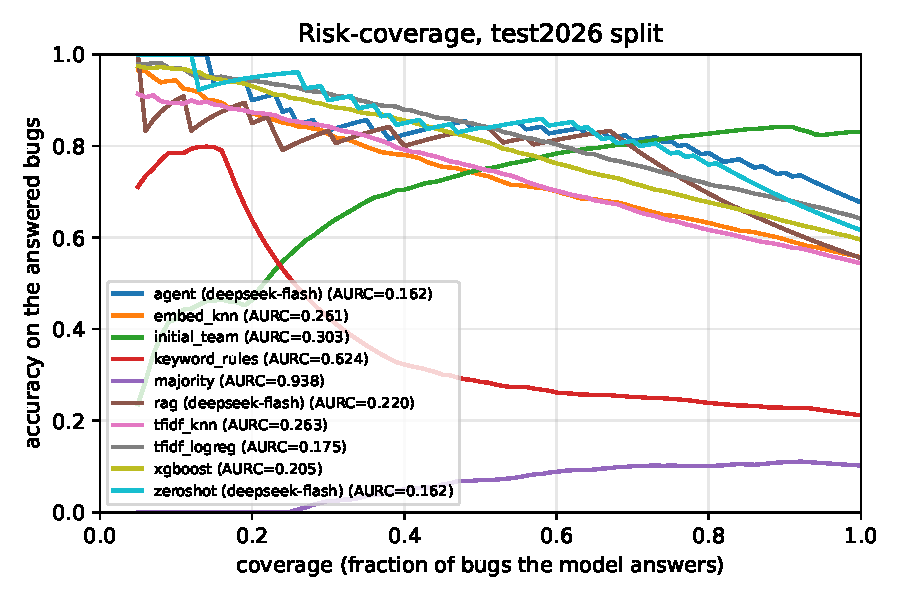
\includegraphics[width=\linewidth]{figures/risk_coverage_test2026.pdf}
\caption{Risk-coverage on the 2026 test period. Source: \texttt{code/make\_figures.py}.}
\label{fig:riskcoverage-test2026}
\end{figure}

\paragraph{Routing accuracy.}
Every LLM condition beats every classical model. The agent reaches \nAgentAcc\% against \nLrAcc\% for
TF-IDF with logistic regression, \nXgbAcc\% for XGBoost and 55.7\% for the embedding $k$NN, and the
advantage survives at the top of the list: \nAgentTop\% top-3 against \nLrTop\%
(Table~\ref{tab:conditions-test2026}). It does not beat the reporter baseline, which stands at
\nRepAcc\%. Taken alone, overall accuracy still argues for leaving the routing to whoever filed the
report.

% Generated by code/make_tables.py from results/metrics_*.json (code/evaluate.py)
\begin{table*}[t]\centering
\caption{Every condition, scored by one evaluator so the risk-coverage curves are directly comparable. Source: \texttt{results/metrics\_*.json}.}
\label{tab:conditions-test2026}
\begin{tabular}{llrrrrrrrrr}
\toprule
Condition & Model & Seed & $n$ & Acc & Macro-F1 & Top-3 & AURC & Acc@80\% & Abstain & \$/bug \\
\midrule
agent & deepseek-flash & 0 & 6{,}347 & 78.9 & 76.0 & 93.5 & 0.077 & 86.2 & 0.3 & 0.00471 \\
embed\_knn & classical & -- & 6{,}347 & 55.7 & 49.4 & 81.0 & 0.253 & 63.2 & 0.0 & -- \\
initial\_team & classical & -- & 6{,}347 & 83.1 & 84.5 & 87.4 & 0.333 & 82.7 & 0.0 & -- \\
keyword\_rules & classical & -- & 6{,}347 & 19.7 & 24.2 & 44.2 & 0.635 & 22.7 & 0.0 & -- \\
majority & classical & -- & 6{,}347 & 9.4 & 0.9 & 35.2 & 0.945 & 10.0 & 0.0 & -- \\
rag & deepseek-flash & 0 & 6{,}347 & 68.0 & 63.3 & 87.7 & 0.176 & 73.7 & 0.3 & 0.00177 \\
tfidf\_knn & classical & -- & 6{,}347 & 53.8 & 49.8 & 77.2 & 0.266 & 61.1 & 0.0 & -- \\
tfidf\_logreg & classical & -- & 6{,}347 & 62.5 & 55.9 & 84.4 & 0.184 & 69.9 & 0.0 & -- \\
xgboost & classical & -- & 6{,}347 & 59.6 & 54.6 & 82.1 & 0.196 & 67.7 & 0.0 & -- \\
zeroshot & deepseek-flash & 0 & 6{,}347 & 70.9 & 63.6 & 88.4 & 0.157 & 76.1 & 0.9 & 0.00143 \\
\bottomrule
\end{tabular}
\end{table*}

% Generated by code/make_tables.py from results/metrics_*.json (test2026).
\begin{table*}[t]\centering
\small
\caption{Cost and latency per bug on the test2026 split. Costs are the recorded API spend at off-peak list price; the classical methods run locally and cost nothing. ``in'' and ``out'' are mean prompt and completion tokens, and ``calls'' the mean number of tool calls per bug. A dash means the quantity does not apply. Source: \texttt{results/metrics\_*.json}; the billed total, including peak-hour calls, is audited by \texttt{code/spend\_report.py} into \texttt{results/spend\_report.json}.}
\label{tab:cost-test2026}
\begin{tabular}{lrrrrrr}
\toprule
Condition & $n$ & \$/bug & in & out & s/bug & calls \\
\midrule
agent (deepseek-flash) & 6{,}347 & 0.0047 & 30214 & 303 & 5.09 & 3.57 \\
zeroshot (deepseek-flash) & 6{,}347 & 0.0014 & 9254 & 66 & 1.77 & 0.00 \\
rag (deepseek-flash) & 6{,}347 & 0.0018 & 11532 & 65 & 1.69 & 0.00 \\
embed\_knn & 6{,}347 & -- & -- & -- & -- & -- \\
initial\_team & 6{,}347 & -- & -- & -- & -- & -- \\
keyword\_rules & 6{,}347 & -- & -- & -- & -- & -- \\
majority & 6{,}347 & -- & -- & -- & -- & -- \\
tfidf\_knn & 6{,}347 & -- & -- & -- & -- & -- \\
tfidf\_logreg & 6{,}347 & -- & -- & -- & -- & -- \\
xgboost & 6{,}347 & -- & -- & -- & -- & -- \\
\bottomrule
\end{tabular}
\end{table*}


\paragraph{What that accuracy costs.}
The gain is not free, and the bill is worth stating rather than leaving in a footnote
(Table~\ref{tab:cost-test2026}). The agent costs \$\nAgentUsd{} per bug against \$\nZSUsd{} for
zero-shot and \$\nRagUsd{} for single-round RAG, and takes \nAgentLat{} seconds per bug against
\nZSLat{} seconds. Most of both is the tool loop: the agent makes \nAgentCalls{} tool calls per bug
on average, which is where its \nAgentInTok{} input tokens per bug come from. In absolute terms this
is cheap --- under half a cent per bug --- so the trade is easy to accept when the reports being
routed are the ambiguous tenth. It would be much harder to justify if the model were mostly
recovering what the reporter already said, which is precisely what the aggregate number rewards.

\paragraph{The subgroup that decides it.}
The picture changes on the bugs whose component was moved away from a concrete one. There the
reporter baseline falls to \nRepSpecAcc\% and TF-IDF with logistic regression to \nLrSpecAcc\%,
while the agent holds \nAgentSpecAcc\% on the \nAgentSpecN{} such bugs it covered:
\nAgentSpecOverLr{} points above the best classical model and \nAgentSpecOverRep{} points above the
baseline. The distance between the two categories is also smallest for the agent ---
\nAgentNeverAcc\% against \nAgentSpecAcc\% --- where the reporter baseline has
\nRepNeverAcc\% against \nRepSpecAcc\%. The practical reading is that a model is worth deploying
only for the fraction of reports whose ownership moved, and that is exactly the fraction overall
accuracy does not isolate.

% Generated by code/make_tables.py from results/metrics_*.json (code/evaluate.py)
\begin{table*}[t]\centering
\caption{Accuracy and confidence-based abstention by ownership-ambiguity category on the full test2026 split. Every classical method is less accurate on \texttt{specific\_reassign} than on \texttt{never\_changed} and abstains no more often there (lift below 1), so its confidence does not track the ambiguity. The agent abstains more often on it (lift 1.21) and is 14.4 points more accurate there than the best classical model. Categories come from \texttt{code/label\_cleaning.py}.}
\label{tab:ambiguity-test2026}
\begin{tabular}{llrrrrrrrr}
\toprule
Condition & Model & Acc never & Acc specific & Gap & Abst.\ specific & Abst.\ never & Lift & Pred=init & Err=init \\
\midrule
agent & deepseek-flash & 80.0 & 71.2 & 8.8 & 22.6 & 19.0 & 1.13 & 41.6 & 49.7 \\
embed\_knn & classical & 55.6 & 51.5 & 4.0 & 18.0 & 20.8 & 0.90 & 34.0 & 24.8 \\
initial\_team & classical & 100.0 & 32.8 & 67.2 & 33.1 & 21.2 & 1.65 & 88.4 & 84.8 \\
keyword\_rules & classical & 19.7 & 21.5 & -1.8 & 15.7 & 20.4 & 0.79 & 11.6 & 4.3 \\
majority & classical & 8.5 & 14.0 & -5.5 & 17.4 & 20.3 & 0.87 & 8.2 & 3.7 \\
rag & deepseek-flash & 68.9 & 61.1 & 7.8 & 17.7 & 19.9 & 0.88 & 39.3 & 37.6 \\
tfidf\_knn & classical & 54.7 & 49.8 & 4.9 & 16.9 & 20.4 & 0.85 & 32.9 & 22.8 \\
tfidf\_logreg & classical & 63.0 & 55.6 & 7.4 & 16.8 & 21.3 & 0.84 & 36.9 & 29.6 \\
xgboost & classical & 60.2 & 52.9 & 7.3 & 13.9 & 21.6 & 0.69 & 35.2 & 27.5 \\
zeroshot & deepseek-flash & 72.4 & 63.7 & 8.7 & 13.9 & 20.5 & 0.69 & 38.1 & 35.3 \\
\bottomrule
\end{tabular}
\end{table*}

% Generated by code/significance.py from results/significance_test2026.json
\begin{table*}[t]\centering
\small
\caption{Pairwise McNemar exact tests on top-1 correctness, test2026 split. Each row uses only the bugs that both conditions answered, so $n$ differs between rows; ``A only'' and ``B only'' count the bugs that only the first and only the second condition got right. Source: \texttt{results/significance\_test2026.json}.}
\label{tab:significance-test2026}
\begin{tabular}{lrrrr}
\toprule
Comparison & $n$ shared & A only & B only & $p$ \\
\midrule
agent@deepseek-flash vs rag@deepseek-flash & 6{,}347 & 978 & 287 & 1.8e-88 \\
agent@deepseek-flash vs zeroshot@deepseek-flash & 6{,}347 & 852 & 346 & 1.1e-49 \\
rag@deepseek-flash vs zeroshot@deepseek-flash & 6{,}347 & 662 & 847 & 2.1e-06 \\
agent@deepseek-flash vs embed\_knn & 6{,}347 & 1{,}765 & 296 & 4.6e-254 \\
agent@deepseek-flash vs initial\_team & 6{,}347 & 767 & 1{,}039 & 1.7e-10 \\
agent@deepseek-flash vs keyword\_rules & 6{,}347 & 3{,}825 & 72 & 0 \\
agent@deepseek-flash vs majority & 6{,}347 & 4{,}470 & 63 & 0 \\
agent@deepseek-flash vs tfidf\_knn & 6{,}347 & 1{,}864 & 273 & 1.2e-290 \\
agent@deepseek-flash vs tfidf\_logreg & 6{,}347 & 1{,}383 & 342 & 3.9e-148 \\
agent@deepseek-flash vs xgboost & 6{,}347 & 1{,}556 & 331 & 2e-189 \\
\bottomrule
\end{tabular}
\end{table*}


\paragraph{Knowing when to decline.}
Ordering the bugs by confidence and answering only the most confident fraction gives the agent the
best risk-coverage curve of any method we evaluate (Figure~\ref{fig:riskcoverage-test2026}): AURC
\nAgentAurc{} against \nLrAurc{} for
logistic regression and \nRepAurc{} for the reporter baseline, and \nAgentCov\% correct on the 80\%
of bugs it chooses to answer. Its abstention rates point the right way and only just: on the
reassigned subgroup it declines \nAgentSpecAbst\% of the time against \nAgentNeverAbst\% elsewhere,
a lift of \nAgentLift, where every classical method does the opposite, declining on the hard bugs at
\nClassicalLiftMin--\nClassicalLiftMax{} times its own average rate. Zero-shot (\nZSLift) and RAG (\nRagLift) fall in between: they
are more accurate than the classical models, but their confidence is, like the classical models',
backwards.

\subsection{Robustness}
\label{sec:robustness}

\paragraph{A second test period.}
The reversal we report is not a property of one data slice. The 2024 test period was collected from
the same tracker two years earlier, and every condition in Table~\ref{tab:periods} runs locally, so
the comparison costs nothing to repeat. The pattern is identical in both periods: the reporter
baseline is the most accurate method overall (80.3\% and \nRepAcc\%), it is exactly right wherever
ownership never moved (100.0\% in both), and it collapses on the bugs whose component was moved away
from a concrete one, falling below TF-IDF with logistic regression --- 28.0\% against 50.9\% in
2024, and \nRepSpecAcc\% against \nLrSpecAcc\% in 2026. What changed between the periods is the size
of the subgroup: the share of bugs whose ownership moved grew from 7.5\% to 10.3\%, so the part
overall accuracy hides is getting larger, not smaller.

% Generated by code/make_tables.py from results/metrics_*.json.
\begin{table*}[t]\centering
\small
\caption{The reversal on two independent test periods. ``Never'' and ``Moved'' are the accuracy on bugs whose component was never reassigned and on bugs whose component was moved away from a concrete one. Both periods come from the same tracker two years apart and the pattern is identical: the reporter baseline wins overall, is perfect where ownership never moved, and collapses where it did, falling below TF-IDF with logistic regression. Source: \texttt{results/metrics\_*.json}, \texttt{results/baselines\_ext\_*.json}.}
\label{tab:periods}
\begin{tabular}{llrrrrr}
\toprule
Period & Condition & $n$ & Acc & Never & Moved & $n$ moved \\
\midrule
2024 & initial\_team & 5{,}469 & 80.3 & 100.0 & 28.0 & 411 \\
 & keyword\_rules & 5{,}469 & 23.6 & 23.8 & 16.5 & 411 \\
 & majority & 5{,}469 & 9.5 & 9.5 & 9.2 & 411 \\
 & tfidf\_knn & 5{,}469 & 54.6 & 56.4 & 42.1 & 411 \\
 & tfidf\_logreg & 5{,}469 & 62.5 & 63.3 & 50.9 & 411 \\
\midrule
2026 & initial\_team & 6{,}347 & 83.1 & 100.0 & 32.8 & 656 \\
 & keyword\_rules & 6{,}347 & 19.7 & 19.7 & 21.5 & 656 \\
 & majority & 6{,}347 & 9.4 & 8.5 & 14.0 & 656 \\
 & tfidf\_knn & 6{,}347 & 53.8 & 54.7 & 49.8 & 656 \\
 & tfidf\_logreg & 6{,}347 & 62.5 & 63.0 & 55.6 & 656 \\
\bottomrule
\end{tabular}
\end{table*}


\paragraph{Labels that had time to settle.}
A bug filed shortly before the freeze could still be reassigned, which would make its label a moving
target as we watch it. The settled subset keeps only bugs filed at least 90 days before the freeze
and repeats the comparison (Table~\ref{tab:ambiguity-test2026-settled}); it is unchanged.
% Generated by code/make_tables.py from results/metrics_*.json (code/evaluate.py)
\begin{table*}[t]\centering
\caption{Accuracy and confidence-based abstention by ownership-ambiguity category on the settled subset, i.e.\ bugs filed at least 90 days before the freeze. Every classical method is less accurate on \texttt{specific\_reassign} than on \texttt{never\_changed} and abstains no more often there (lift below 1), so its confidence does not track the ambiguity. The agent abstains more often on it (lift 1.21) and is 14.4 points more accurate there than the best classical model. Categories come from \texttt{code/label\_cleaning.py}.}
\label{tab:ambiguity-test2026-settled}
\begin{tabular}{llrrrrrrrr}
\toprule
Condition & Model & Acc never & Acc specific & Gap & Abst.\ specific & Abst.\ never & Lift & Pred=init & Err=init \\
\midrule
keyword\_rules & classical & 21.2 & 22.6 & -1.4 & 17.9 & 20.1 & 0.89 & 12.4 & 4.6 \\
majority & classical & 9.3 & 14.9 & -5.6 & 18.3 & 20.0 & 0.91 & 9.2 & 4.2 \\
tfidf\_knn & classical & 55.1 & 51.6 & 3.5 & 17.5 & 20.5 & 0.88 & 33.0 & 21.0 \\
tfidf\_logreg & classical & 64.4 & 58.8 & 5.6 & 18.3 & 21.2 & 0.91 & 37.7 & 28.3 \\
\bottomrule
\end{tabular}
\end{table*}


\section{Error analysis}
\label{sec:errors}

% DRAFT for author review (rule 7). Every number below appears in
% Table~\ref{tab:confusions-test2026}, Table~\ref{tab:ambiguity-test2026} or
% Table~\ref{tab:headtohead-test2026}.

\paragraph{Where the mistakes go.}
The mistakes of TF-IDF with logistic regression are not spread evenly over the 20 teams.
Table~\ref{tab:confusions-test2026} lists its ten most frequent confusions, and the largest by a
wide margin is Frontend against Search Next Generation: 217 bugs owned by Frontend are answered
with Search Next Generation, and 87 go the other way. The next groups are Layout against GFX
(65 and 60) and DOM Core against Layout (64 and 47). Each of these is a pair of teams whose
reports describe the same user-visible symptoms, which suggests the remaining error is a
vocabulary problem rather than a coverage problem: more training data of the same kind would not
separate them.

\paragraph{Where the agent loses.}
Comparing two accuracy percentages cannot say where a difference comes from, so
Table~\ref{tab:headtohead-test2026} counts the disagreements directly, over the \nSharedN{} bugs
that both the agent and TF-IDF with logistic regression answered. The agent is right where logistic
regression is wrong on \nAgentOnly{} bugs and the reverse on \nLrOnly{}. The margin is about the same
in both ownership categories --- \nNetNever{} points on the bugs whose ownership never moved and
\nNetMoved{} on the ones where it did --- which says the agent is not merely better on the hard
subgroup but better everywhere, as one would expect from a model that reads more of the report. The
subgroup still matters, for a different reason: it is where the reporter baseline fails, and no
aggregate accuracy reveals that. Where the agent does lose, the losses follow team size rather than
area. Frontend (\nLossOne{} bugs), DOM Core (\nLossTwo{}) and Search Next Generation (\nLossThree{})
are also the three teams with the most bugs in the test period, so the losses are a volume effect
rather than a gap in one part of the tracker.

% Generated by code/agent_vs_baseline.py from llm_agent_deepseek-flash_test2026_disabled_n6347_seed0.jsonl and pred_tfidf_logreg_test2026.jsonl.
\begin{table*}[t]\centering
\small
\caption{Where the agent and TF-IDF with logistic regression disagree, over the 6{,}347 bugs both answered. ``Net'' is the agent's advantage in accuracy points on that row. The advantage is roughly twice as large per bug where ownership moved, and the teams the agent loses to are the largest ones, so the losses are a volume effect rather than a gap in one area. Source: \texttt{llm\_agent\_deepseek-flash\_test2026\_disabled\_n6347\_seed0.jsonl}, \texttt{pred\_tfidf\_logreg\_test2026.jsonl}.}
\label{tab:headtohead-test2026}
\begin{tabular}{lrrrr}
\toprule
Subset & $n$ & Agent only & LR only & Net \\
\midrule
All shared bugs & 6{,}347 & 1{,}383 & 342 & +16.4 \\
Ownership never moved & 4{,}958 & 1{,}094 & 253 & +17.0 \\
Ownership moved away & 656 & 138 & 36 & +15.6 \\
\bottomrule
\end{tabular}
\end{table*}


\paragraph{A strong model is pulled towards the answer that was overruled.}
Section~\ref{sec:data} labels every bug by whether its component moved. Where it did not, the
reporter's initial team is by definition the final team, so reproducing it can never be a mistake.
Where the bug was reassigned away from a concrete component the picture reverses: the last column
of Table~\ref{tab:ambiguity-test2026} gives the share of a model's mistakes on that subgroup that
land on the team the reporter first filed under, i.e. exactly the choice that was overruled.
TF-IDF with logistic regression does so in 29.6\% of its mistakes there, XGBoost in 27.5\%, the
sentence-embedding $k$NN in 24.8\% and TF-IDF $k$NN in 22.8\%. The ordering follows model quality
exactly (53.8\%, 55.7\%, 59.6\% and 62.5\% overall accuracy in the same order, from
Table~\ref{tab:conditions-test2026}): the better the model, the more of its remaining errors are
the reporter's original choice. A weak model fails for its own reasons; a strong one converges on
what the reporter said before a triager moved the bug.

This is the behaviour the LLM conditions were meant to avoid: a model that only reads the report can
recover the pre-reassignment answer, because that answer is written into the report. The answer from
Section~\ref{sec:results} is that the agent does not avoid it. On the reassigned subgroup
\nAgentErrInit\% of the agent's mistakes land on the team the reporter first filed under, which is
higher than any classical model and well above the \nLrErrInit\% of logistic regression. What the
agent buys is not immunity to the reporter's original choice but a higher rate of getting past it:
it reaches \nAgentSpecAcc\% on that subgroup against \nLrSpecAcc\%, so it recovers from the
superseded answer more often rather than never falling for it. That distinction matters for anyone
deploying this: the agent does not stop being misled by the report, it just notices more often.

% Generated by code/make_tables.py from results/metrics_tfidf_logreg_test2026.json
\begin{table}[t]\centering
\small
\caption{The ten most frequent confusions of \texttt{tfidf\_logreg} on the test2026 split: the team that owns the bug, and the team the model named first. Source: \texttt{results/metrics\_tfidf\_logreg\_test2026.json} (\texttt{code/evaluate.py}).}
\label{tab:confusions-test2026}
\begin{tabular}{llr}
\toprule
True team & Predicted first & n \\
\midrule
Frontend & Search Next Generation & 217 \\
Search Next Generation & Frontend & 87 \\
Layout & GFX & 65 \\
DOM Core & Layout & 64 \\
GFX & Layout & 60 \\
Frontend & OS Integration & 59 \\
Media & GFX & 58 \\
Frontend & Layout & 47 \\
Layout & DOM Core & 47 \\
OS Integration & GFX & 41 \\
\bottomrule
\end{tabular}
\end{table}


\section{Limitations}
\label{sec:limitations}

% DRAFT for author review (rule 7). Statements here are about how the data was built and what was
% measured; nothing is claimed that a script in code/ does not do.

\paragraph{The team mapping is current, not historical.}
The Bugzilla API does not expose the component-to-team mapping that was in force when a bug was
filed, so we label every bug with today's ownership. A bug that moved component for organisational
reasons is therefore labelled by current ownership, and a team renamed or split since 2022 is
invisible to us. This is the main threat to construct validity in this paper, and it is the reason
we report two test periods rather than one.

\paragraph{Reassignment is a proxy for ambiguity, not a measurement of it.}
We infer ownership ambiguity from the fact that a bug's component changed. Some of those moves are
routine: a triager can move a report to a more specific component without anyone disagreeing about
which team owns it. We separate the inbox cases and the automation cases out of the candidate set
for exactly this reason, but the residual group is still a proxy, so we treat the per-category
numbers as descriptive rather than as a gold-standard evaluation.

\paragraph{The reporter baseline is not a human baseline.}
We do not model who filed each report. Many Bugzilla reports come from developers or from
automation rather than from a user meeting the product for the first time, so trusting the initial
component is an upper bound on what "trust the filer" can achieve, not a model of a human triager.

\paragraph{One project, one split, one model family.}
All numbers come from Mozilla Bugzilla, with a single train/test split and a 20-team label space
chosen by frequency. The settled subset is a stability check on the labels, not cross-validation
across time. The LLM conditions use one provider, so model quality and prompt design cannot be
separated from each other.

\paragraph{Costs and token counts are estimates.}
Dollar figures apply list prices to token counts produced by a proxy tokenizer rather than by the
provider's own tokenizer, and prompt caching, off-peak pricing and retries all move the real bill.
Latency includes network time. We report them to bound the cost of the method, not as a
measurement of it.

\section{Reproducibility}
\label{sec:repro}
The whole pipeline runs from one command, \texttt{code/run\_all.py}, which calls the other scripts
in order and reports what each one wrote; the paid steps run only when it is given
\texttt{--with-llm} and an API key is present. Data is pulled from the public Bugzilla REST API by
\texttt{code/fetch\_period.py}, so the corpus can be rebuilt from scratch rather than taken on
trust. \texttt{code/requirements.txt} pins every dependency.

One discrepancy is worth recording. The TF-IDF with logistic regression baseline scores 62.443\% on
the 2024 test period on the machine where the first results were produced and 62.534\% on the
machine used here, on the same dataset; we attribute the difference to library versions. The
original outputs are kept in \texttt{results/} next to the new ones instead of being overwritten,
and the pinned versions in \texttt{code/requirements.txt} are what the reported numbers were
produced with.

Every model response is cached on disk under a key derived from the exact request payload, so a run
can be interrupted and resumed without paying for the same request twice, and a spend guard aborts
a run that exceeds its budget. Given that cache, prompt construction, response parsing and scoring
are deterministic.

\section{Conclusion}
A router is usually judged by how often it names the right team. On this benchmark that measure
picks the wrong winner: predicting the team that owns the component the reporter already chose
scores \nRepAcc\%, better than any model, but it collapses to \nRepSpecAcc\% on the reports whose
ownership actually moved, which is the only subgroup where routing is still undecided. A tool-using
LLM agent takes that subgroup to \nAgentSpecAcc\%, \nAgentSpecOverLr{} points above the best
classical model, and it is the one learned method whose confidence is higher there than elsewhere,
so it can be spent selectively where a human reviewer is worth the most. Aggregate accuracy hides
all of this, and we would suggest that routing results be reported per ownership category from now
on.

Two threats to validity remain. The component-to-team mapping we use is the current one, not the
historical one, so a bug whose component changed for organisational rather than technical reasons is
labelled by today's ownership; an organisational mapping would be a better label. And the agent is
priced in tokens here; whether it pays for itself depends on how much triage time it saves, which a
token bill does not measure.

\section*{Acknowledgment}
% Required by the ICST 2027 generative-AI policy, and true of the ISSTA and arXiv builds too, so it
% lives in the shared body rather than in one format layer. That policy asks for the tools, the
% affected sections and the extent of use; keep all three if this is edited.
The author used an AI coding assistant --- an agentic tool loop driving DeepSeek and Gemini language
models --- while preparing this paper, and remains solely responsible for all content, claims and
references. The assistant drafted and revised the prose of every section of the manuscript, and wrote
the analysis scripts in the replication package; the tables and figures are produced by those scripts
from recorded results rather than composed by the assistant, and every reference was checked against
the published record. The language models evaluated in Section~\ref{sec:setup} are the object of
study rather than writing assistance, and are described there.
\bibliographystyle{ACM-Reference-Format}
% paper/build.py copies ../../../shared/references.bib to paper/references.bib before compiling,
% because Tectonic refuses to read files above the main file's directory. With a full TeX
% distribution that supports parent paths you can point this straight at
% ../../../shared/references instead.
\bibliography{references}

\end{document}
